\documentclass[aspectratio=169]{beamer}

% Minimal theme
\usetheme{default}
\usecolortheme{dove}

% Remove navigation symbols
\setbeamertemplate{navigation symbols}{}
\setbeamertemplate{footline}{%
  \hfill{\large\insertframenumber\,/\,\inserttotalframenumber}\hspace{0.8em}\vspace{0.5em}%
}

% Colors
\definecolor{popblue}{RGB}{52, 101, 164}
\definecolor{sampred}{RGB}{204, 0, 0}
\definecolor{paramgreen}{RGB}{0, 140, 70}
\definecolor{lightbg}{RGB}{245, 245, 250}
\definecolor{warnred}{RGB}{180, 40, 40}
\definecolor{orange1}{RGB}{220, 120, 0}
\definecolor{violet1}{RGB}{120, 50, 160}

\setbeamercolor{frametitle}{fg=popblue}
\setbeamercolor{title}{fg=popblue}

% Packages
\usepackage{pgfplots}
\usepackage{tikz}
\usetikzlibrary{shapes, arrows.meta, positioning, calc, decorations.pathreplacing, patterns, fit}
\pgfplotsset{compat=1.18}
\usepackage{amsmath, amssymb}
\usepackage{array}
\usepackage[T1]{fontenc}

\title{Reinforcement Learning for Language Models}
\subtitle{MDPs $\cdot$ Q-Learning $\cdot$ Policy Gradients $\cdot$ RLHF $\cdot$ PPO $\cdot$ DPO $\cdot$ GRPO}
\date{}

\begin{document}

% ============================================================
% TITLE
% ============================================================
\begin{frame}
\titlepage
\end{frame}

% ============================================================
% WHY RL FOR NLP?
% ============================================================
\begin{frame}
\frametitle{Why reinforcement learning for NLP?}

\begin{center}
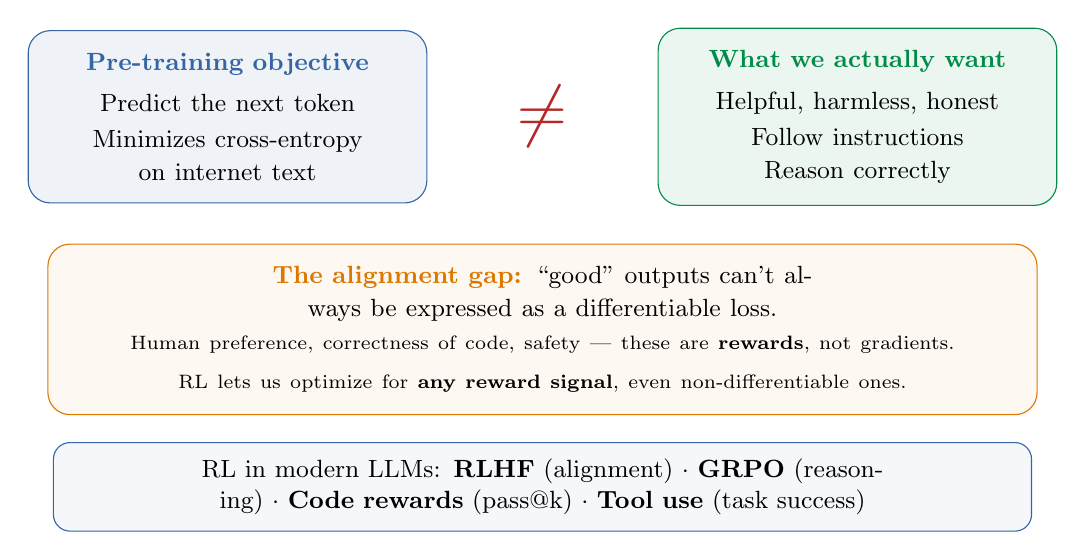
\begin{tikzpicture}
  % The gap
  \node[draw=popblue, fill=popblue!8, rounded corners=8pt, text width=4.5cm, align=center, inner sep=8pt] at (-4, 2.2) {
    {\small\bfseries\textcolor{popblue}{Pre-training objective}}\\[4pt]
    {\small Predict the next token\\[2pt]
    Minimizes cross-entropy\\on internet text}
  };

  \node[font=\Huge, text=warnred] at (0, 2.2) {$\neq$};

  \node[draw=paramgreen, fill=paramgreen!8, rounded corners=8pt, text width=4.5cm, align=center, inner sep=8pt] at (4, 2.2) {
    {\small\bfseries\textcolor{paramgreen}{What we actually want}}\\[4pt]
    {\small Helpful, harmless, honest\\[2pt]
    Follow instructions\\Reason correctly}
  };

  % Why RL?
  \node[draw=orange1, fill=orange1!5, rounded corners=8pt, text width=12cm, align=center, inner sep=8pt] at (0, -0.5) {
    {\small\bfseries\textcolor{orange1}{The alignment gap:}} {\small ``good'' outputs can't always be expressed as a differentiable loss.}\\[4pt]
    {\scriptsize Human preference, correctness of code, safety --- these are \textbf{rewards}, not gradients.\\[2pt]
    RL lets us optimize for \textbf{any reward signal}, even non-differentiable ones.}
  };

  % Where RL appears
  \node[draw=popblue, fill=popblue!5, rounded corners=6pt, text width=12cm, align=center, inner sep=6pt, font=\small] at (0, -2.5) {
    RL in modern LLMs: \textbf{RLHF} (alignment) $\cdot$ \textbf{GRPO} (reasoning) $\cdot$
    \textbf{Code rewards} (pass@k) $\cdot$ \textbf{Tool use} (task success)
  };
\end{tikzpicture}
\end{center}
\end{frame}

% ============================================================
% PART I: CLASSICAL RL FOUNDATIONS
% ============================================================
\begin{frame}
\begin{center}
\vspace{2cm}
{\Huge \textcolor{popblue}{Part I}}

\vspace{0.5cm}
{\Large Classical RL Foundations}

\vspace{0.3cm}
{\normalsize MDPs $\cdot$ Value Functions $\cdot$ Q-Learning $\cdot$ Policy Gradients}
\end{center}
\end{frame}

% ============================================================
% THE RL FRAMEWORK: MDP
% ============================================================
\begin{frame}
\frametitle{The RL framework: Markov Decision Process}

\begin{center}
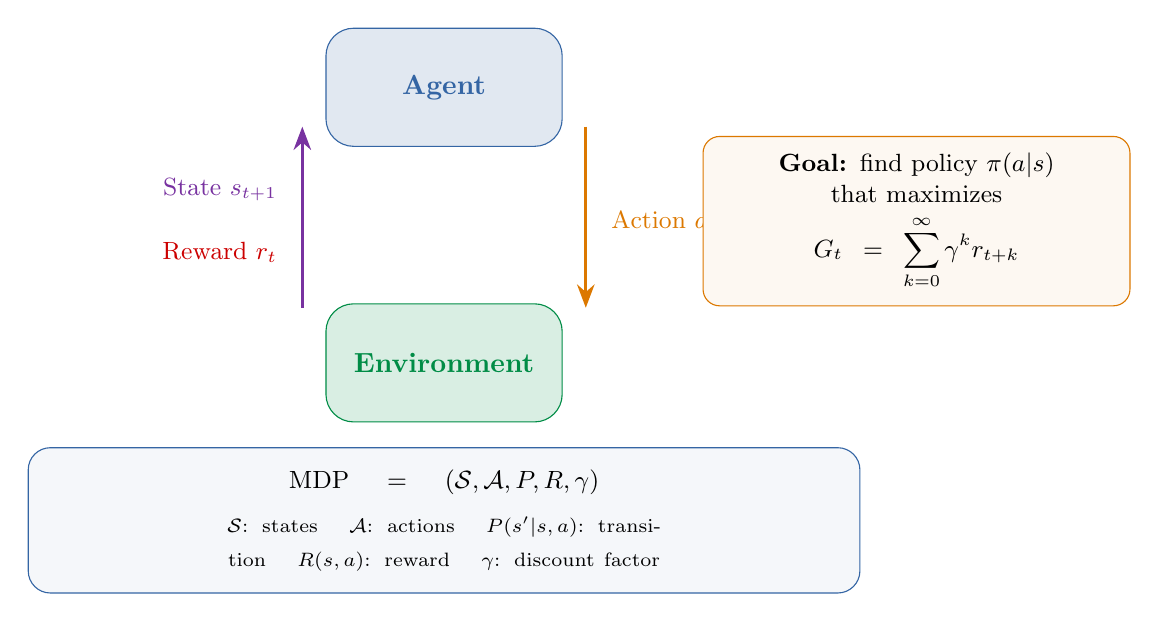
\begin{tikzpicture}
  % Agent-environment loop
  \node[draw=popblue, fill=popblue!15, rounded corners=10pt, minimum width=3cm, minimum height=1.5cm, font=\normalsize\bfseries, text=popblue] (agent) at (0, 2) {Agent};
  \node[draw=paramgreen, fill=paramgreen!15, rounded corners=10pt, minimum width=3cm, minimum height=1.5cm, font=\normalsize\bfseries, text=paramgreen] (env) at (0, -1.5) {Environment};

  % Action arrow (right side)
  \draw[-Stealth, very thick, orange1] (1.8, 1.5) -- (1.8, -0.8);
  \node[font=\small, text=orange1, right] at (2, 0.3) {Action $a_t$};

  % State + Reward arrow (left side)
  \draw[-Stealth, very thick, violet1] (-1.8, -0.8) -- (-1.8, 1.5);
  \node[font=\small, text=violet1, left] at (-2, 0.7) {State $s_{t+1}$};
  \node[font=\small, text=sampred, left] at (-2, -0.1) {Reward $r_t$};

  % MDP tuple
  \node[draw=popblue, fill=popblue!5, rounded corners=8pt, text width=10cm, align=center, inner sep=8pt] at (0, -3.5) {
    {\small $\text{MDP} = (\mathcal{S}, \mathcal{A}, P, R, \gamma)$}\\[4pt]
    {\scriptsize $\mathcal{S}$: states \quad $\mathcal{A}$: actions \quad $P(s'|s,a)$: transition \quad $R(s,a)$: reward \quad $\gamma$: discount factor}
  };

  % Goal
  \node[draw=orange1, fill=orange1!5, rounded corners=6pt, text width=5cm, align=center, inner sep=6pt, font=\small] at (6, 0.3) {
    \textbf{Goal:} find policy $\pi(a|s)$\\that maximizes\\[4pt]
    $\displaystyle G_t = \sum_{k=0}^{\infty} \gamma^k r_{t+k}$
  };
\end{tikzpicture}
\end{center}
\end{frame}

% ============================================================
% VALUE FUNCTIONS
% ============================================================
\begin{frame}
\frametitle{Value functions}

\begin{center}
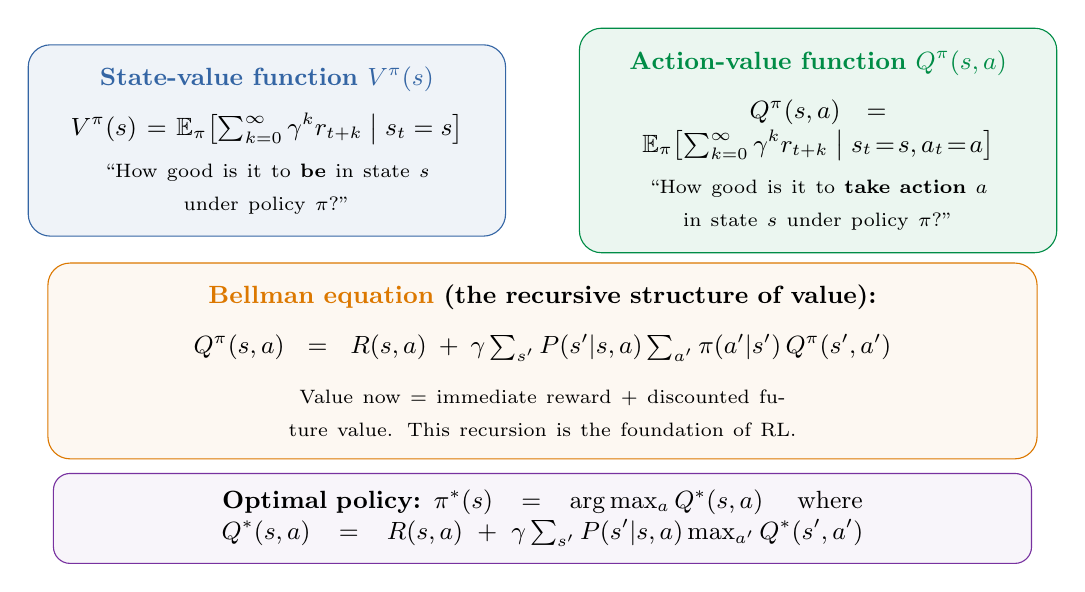
\begin{tikzpicture}
  % State-value function
  \node[draw=popblue, fill=popblue!8, rounded corners=8pt, text width=5.5cm, align=center, inner sep=8pt] at (-3.5, 2) {
    {\small\bfseries\textcolor{popblue}{State-value function $V^\pi(s)$}}\\[6pt]
    {\small $V^\pi(s) = \mathbb{E}_\pi\!\left[\sum_{k=0}^{\infty} \gamma^k r_{t+k} \;\middle|\; s_t = s\right]$}\\[6pt]
    {\scriptsize ``How good is it to \textbf{be} in state $s$\\under policy $\pi$?''}
  };

  % Action-value function
  \node[draw=paramgreen, fill=paramgreen!8, rounded corners=8pt, text width=5.5cm, align=center, inner sep=8pt] at (3.5, 2) {
    {\small\bfseries\textcolor{paramgreen}{Action-value function $Q^\pi(s, a)$}}\\[6pt]
    {\small $Q^\pi(s, a) = \mathbb{E}_\pi\!\left[\sum_{k=0}^{\infty} \gamma^k r_{t+k} \;\middle|\; s_t\!=\!s, a_t\!=\!a\right]$}\\[6pt]
    {\scriptsize ``How good is it to \textbf{take action $a$}\\in state $s$ under policy $\pi$?''}
  };

  % Bellman equation
  \node[draw=orange1, fill=orange1!5, rounded corners=8pt, text width=12cm, align=center, inner sep=8pt] at (0, -0.8) {
    {\small\bfseries\textcolor{orange1}{Bellman equation} (the recursive structure of value):}\\[6pt]
    {\small $Q^\pi(s, a) = R(s, a) + \gamma \sum_{s'} P(s'|s,a) \sum_{a'} \pi(a'|s') \, Q^\pi(s', a')$}\\[6pt]
    {\scriptsize Value now $=$ immediate reward $+$ discounted future value. This recursion is the foundation of RL.}
  };

  % Optimal
  \node[draw=violet1, fill=violet1!5, rounded corners=6pt, text width=12cm, align=center, inner sep=6pt, font=\small] at (0, -2.8) {
    \textbf{Optimal policy:} $\pi^*(s) = \arg\max_a Q^*(s, a)$ \quad where \quad
    $Q^*(s, a) = R(s, a) + \gamma \sum_{s'} P(s'|s,a) \max_{a'} Q^*(s', a')$
  };
\end{tikzpicture}
\end{center}
\end{frame}

% ============================================================
% Q-LEARNING
% ============================================================
\begin{frame}
\frametitle{Q-Learning}

\begin{center}
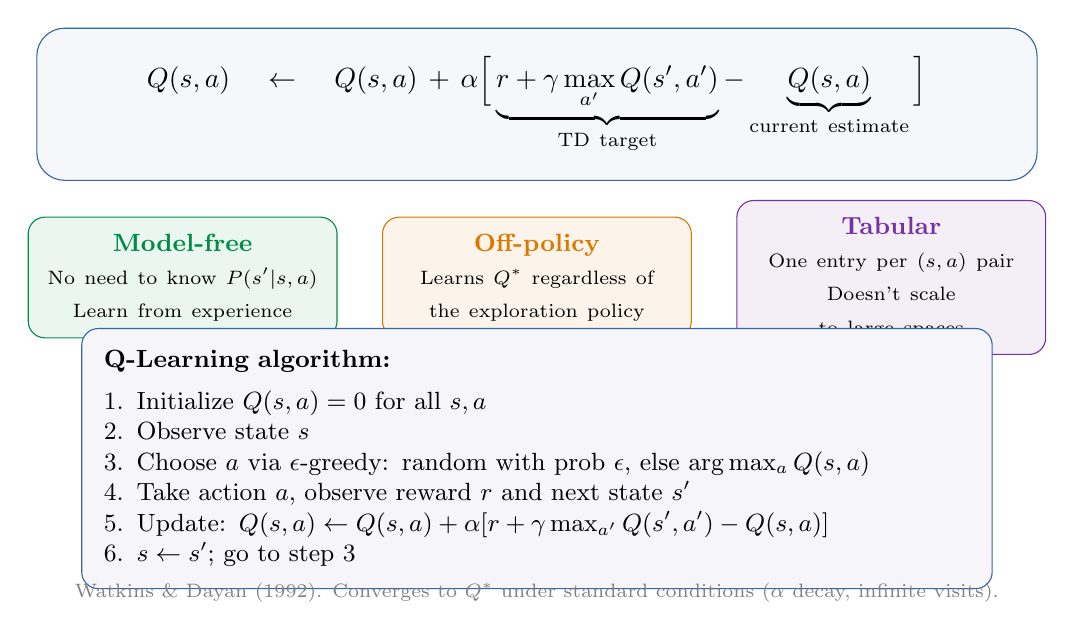
\begin{tikzpicture}
  % The update rule
  \node[draw=popblue, fill=popblue!5, rounded corners=10pt, text width=12cm, align=center, inner sep=10pt] at (0, 3) {
    {\normalsize $Q(s, a) \;\leftarrow\; Q(s, a) + \alpha \Big[\underbrace{r + \gamma \max_{a'} Q(s', a')}_{\text{TD target}} - \underbrace{Q(s, a)}_{\text{current estimate}}\Big]$}
  };

  % Key properties
  \node[draw=paramgreen, fill=paramgreen!8, rounded corners=6pt, text width=3.5cm, align=center, inner sep=6pt] at (-4.5, 0.8) {
    {\small\bfseries\textcolor{paramgreen}{Model-free}}\\[4pt]
    {\scriptsize No need to know $P(s'|s,a)$\\Learn from experience}
  };

  \node[draw=orange1, fill=orange1!8, rounded corners=6pt, text width=3.5cm, align=center, inner sep=6pt] at (0, 0.8) {
    {\small\bfseries\textcolor{orange1}{Off-policy}}\\[4pt]
    {\scriptsize Learns $Q^*$ regardless of\\the exploration policy}
  };

  \node[draw=violet1, fill=violet1!8, rounded corners=6pt, text width=3.5cm, align=center, inner sep=6pt] at (4.5, 0.8) {
    {\small\bfseries\textcolor{violet1}{Tabular}}\\[4pt]
    {\scriptsize One entry per $(s, a)$ pair\\Doesn't scale to large spaces}
  };

  % Algorithm
  \node[draw=popblue, fill=lightbg, rounded corners=6pt, text width=11cm, align=left, inner sep=8pt, font=\small] at (0, -1.5) {
    \textbf{Q-Learning algorithm:}\\[4pt]
    1. Initialize $Q(s, a) = 0$ for all $s, a$\\
    2. Observe state $s$\\
    3. Choose $a$ via $\epsilon$-greedy: random with prob $\epsilon$, else $\arg\max_a Q(s,a)$\\
    4. Take action $a$, observe reward $r$ and next state $s'$\\
    5. Update: $Q(s,a) \leftarrow Q(s,a) + \alpha[r + \gamma \max_{a'} Q(s',a') - Q(s,a)]$\\
    6. $s \leftarrow s'$; go to step 3
  };

  \node[font=\scriptsize, text=gray] at (0, -3.2) {Watkins \& Dayan (1992). Converges to $Q^*$ under standard conditions ($\alpha$ decay, infinite visits).};
\end{tikzpicture}
\end{center}
\end{frame}

% ============================================================
% DEEP Q-NETWORKS (DQN)
% ============================================================
\begin{frame}
\frametitle{Deep Q-Networks (DQN)}

\begin{center}
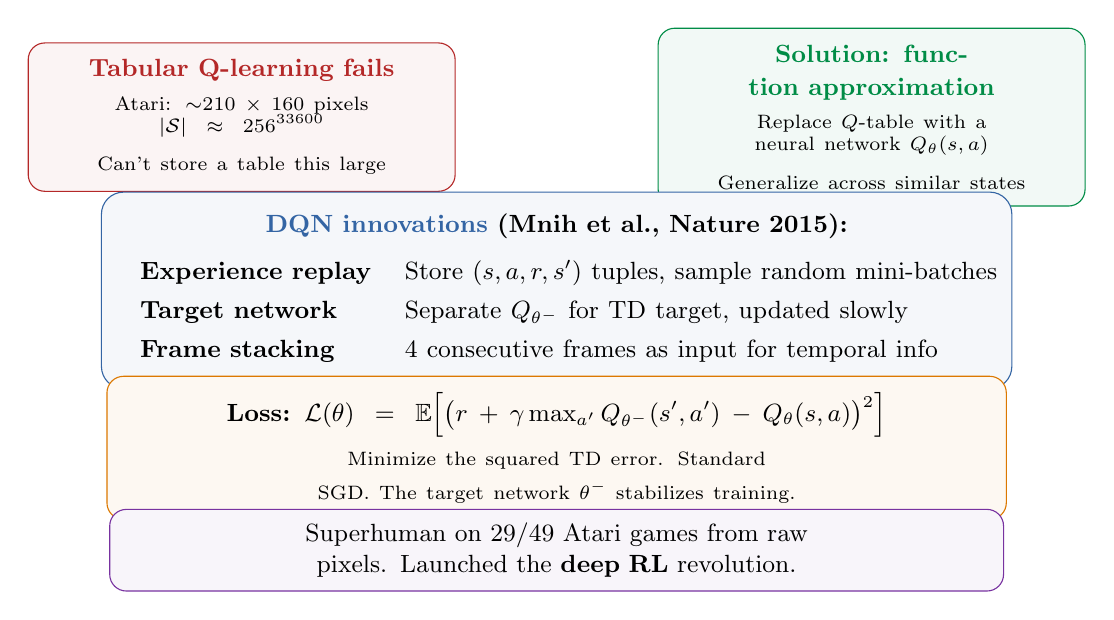
\begin{tikzpicture}
  % Problem with tabular
  \node[draw=warnred, fill=warnred!5, rounded corners=6pt, text width=5cm, align=center, inner sep=6pt] at (-4, 2.5) {
    {\small\bfseries\textcolor{warnred}{Tabular Q-learning fails}}\\[4pt]
    {\scriptsize Atari: $\sim$210 $\times$ 160 pixels\\
    $|\mathcal{S}| \approx 256^{33600}$\\[2pt]
    Can't store a table this large}
  };

  % Solution
  \node[draw=paramgreen, fill=paramgreen!5, rounded corners=6pt, text width=5cm, align=center, inner sep=6pt] at (4, 2.5) {
    {\small\bfseries\textcolor{paramgreen}{Solution: function approximation}}\\[4pt]
    {\scriptsize Replace $Q$-table with a\\neural network $Q_\theta(s, a)$\\[2pt]
    Generalize across similar states}
  };

  % DQN innovations
  \node[draw=popblue, fill=popblue!5, rounded corners=8pt, text width=11cm, align=center, inner sep=8pt] at (0, 0.3) {
    {\small\bfseries\textcolor{popblue}{DQN innovations} (Mnih et al., Nature 2015):}\\[6pt]
    {\small
    \begin{tabular}{l l}
      \textbf{Experience replay} & Store $(s, a, r, s')$ tuples, sample random mini-batches \\[3pt]
      \textbf{Target network} & Separate $Q_{\theta^-}$ for TD target, updated slowly \\[3pt]
      \textbf{Frame stacking} & 4 consecutive frames as input for temporal info
    \end{tabular}
    }
  };

  % Loss
  \node[draw=orange1, fill=orange1!5, rounded corners=6pt, text width=11cm, align=center, inner sep=6pt] at (0, -1.7) {
    {\small \textbf{Loss:} $\mathcal{L}(\theta) = \mathbb{E}\Big[\big(r + \gamma \max_{a'} Q_{\theta^-}(s', a') - Q_\theta(s, a)\big)^2\Big]$}\\[4pt]
    {\scriptsize Minimize the squared TD error. Standard SGD. The target network $\theta^-$ stabilizes training.}
  };

  % Impact
  \node[draw=violet1, fill=violet1!5, rounded corners=6pt, text width=11cm, align=center, inner sep=5pt, font=\small] at (0, -3) {
    Superhuman on 29/49 Atari games from raw pixels. Launched the \textbf{deep RL} revolution.
  };
\end{tikzpicture}
\end{center}
\end{frame}

% ============================================================
% POLICY GRADIENT METHODS
% ============================================================
\begin{frame}
\frametitle{Policy gradient methods}

\begin{center}
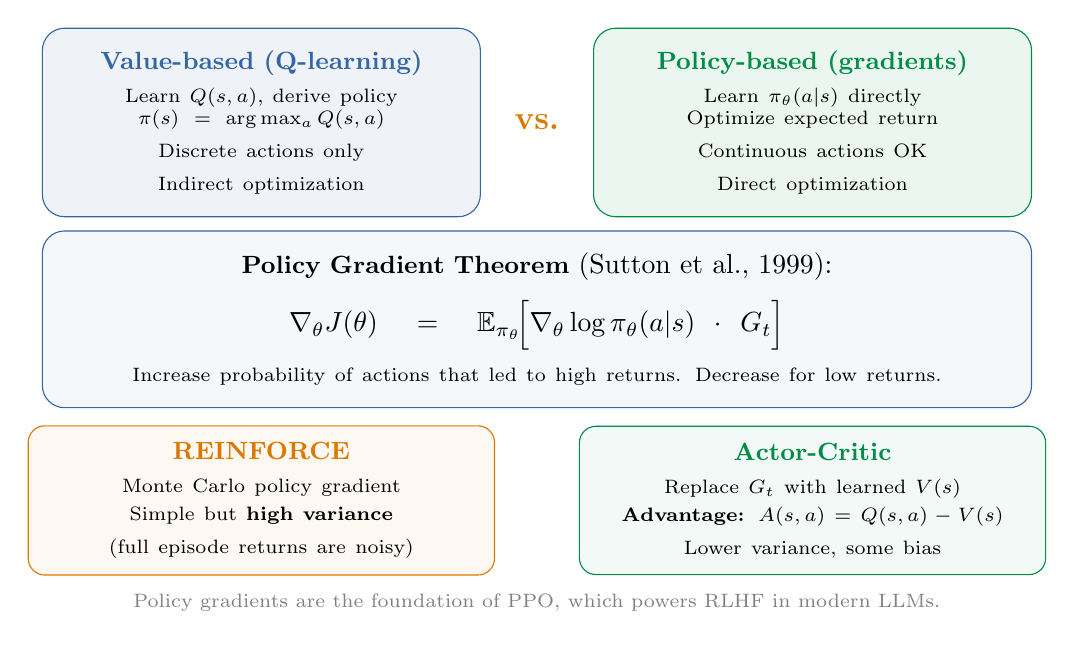
\begin{tikzpicture}
  % Two approaches
  \node[draw=popblue, fill=popblue!8, rounded corners=8pt, text width=5cm, align=center, inner sep=8pt] at (-3.5, 2.8) {
    {\small\bfseries\textcolor{popblue}{Value-based (Q-learning)}}\\[4pt]
    {\scriptsize Learn $Q(s,a)$, derive policy\\$\pi(s) = \arg\max_a Q(s,a)$\\[4pt]
    Discrete actions only\\Indirect optimization}
  };

  \node[font=\large\bfseries, text=orange1] at (0, 2.8) {vs.};

  \node[draw=paramgreen, fill=paramgreen!8, rounded corners=8pt, text width=5cm, align=center, inner sep=8pt] at (3.5, 2.8) {
    {\small\bfseries\textcolor{paramgreen}{Policy-based (gradients)}}\\[4pt]
    {\scriptsize Learn $\pi_\theta(a|s)$ directly\\Optimize expected return\\[4pt]
    Continuous actions OK\\Direct optimization}
  };

  % REINFORCE
  \node[draw=popblue, fill=popblue!5, rounded corners=8pt, text width=12cm, align=center, inner sep=8pt] at (0, 0.3) {
    {\small\bfseries Policy Gradient Theorem} (Sutton et al., 1999):\\[6pt]
    {\normalsize $\nabla_\theta J(\theta) = \mathbb{E}_{\pi_\theta}\!\Big[\nabla_\theta \log \pi_\theta(a|s) \cdot G_t\Big]$}\\[6pt]
    {\scriptsize Increase probability of actions that led to high returns. Decrease for low returns.}
  };

  % REINFORCE algorithm
  \node[draw=orange1, fill=orange1!5, rounded corners=6pt, text width=5.5cm, align=center, inner sep=6pt] at (-3.5, -2) {
    {\small\bfseries\textcolor{orange1}{REINFORCE}}\\[4pt]
    {\scriptsize Monte Carlo policy gradient\\[2pt]
    Simple but \textbf{high variance}\\(full episode returns are noisy)}
  };

  % Actor-Critic
  \node[draw=paramgreen, fill=paramgreen!5, rounded corners=6pt, text width=5.5cm, align=center, inner sep=6pt] at (3.5, -2) {
    {\small\bfseries\textcolor{paramgreen}{Actor-Critic}}\\[4pt]
    {\scriptsize Replace $G_t$ with learned $V(s)$\\[2pt]
    \textbf{Advantage:} $A(s,a) = Q(s,a) - V(s)$\\Lower variance, some bias}
  };

  \node[font=\scriptsize, text=gray] at (0, -3.3) {Policy gradients are the foundation of PPO, which powers RLHF in modern LLMs.};
\end{tikzpicture}
\end{center}
\end{frame}

% ============================================================
% PPO: PROXIMAL POLICY OPTIMIZATION
% ============================================================
\begin{frame}
\frametitle{PPO: Proximal Policy Optimization}

\begin{center}
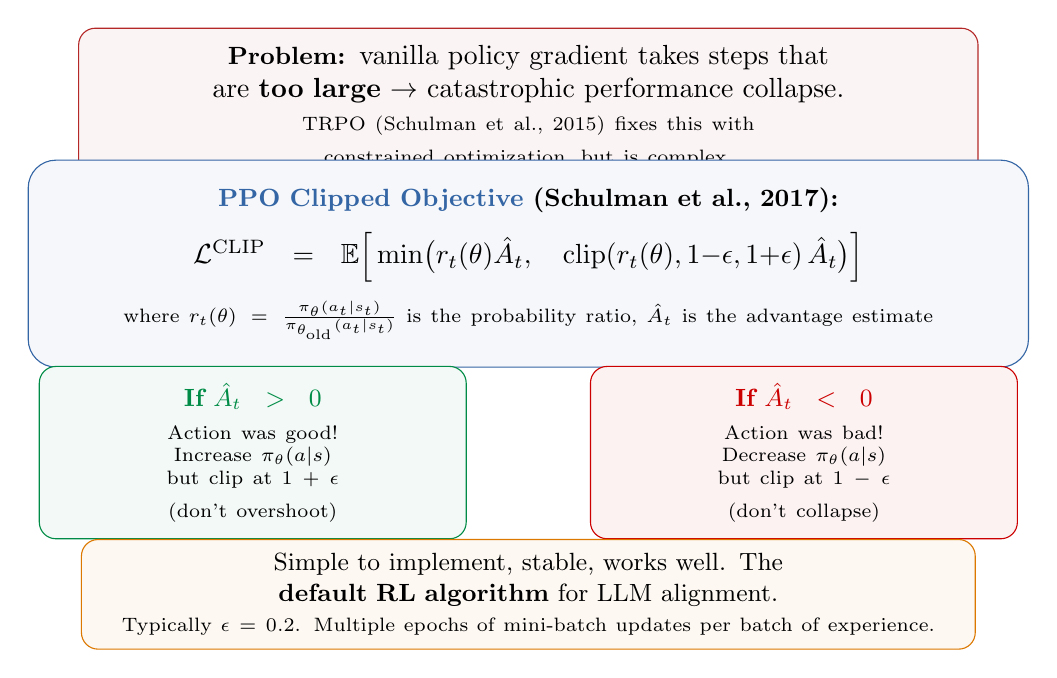
\begin{tikzpicture}
  % Problem
  \node[draw=warnred, fill=warnred!5, rounded corners=6pt, text width=11cm, align=center, inner sep=6pt] at (0, 3.2) {
    {\small\bfseries Problem:} vanilla policy gradient takes steps that are \textbf{too large} $\to$ catastrophic performance collapse.\\
    {\scriptsize TRPO (Schulman et al., 2015) fixes this with constrained optimization, but is complex.}
  };

  % PPO objective
  \node[draw=popblue, fill=popblue!5, rounded corners=10pt, text width=12cm, align=center, inner sep=10pt] at (0, 1.2) {
    {\small\bfseries\textcolor{popblue}{PPO Clipped Objective} (Schulman et al., 2017):}\\[6pt]
    {\normalsize $\mathcal{L}^{\text{CLIP}} = \mathbb{E}\Big[\min\!\big(r_t(\theta) \hat{A}_t, \;\text{clip}(r_t(\theta), 1{-}\epsilon, 1{+}\epsilon)\,\hat{A}_t\big)\Big]$}\\[6pt]
    {\scriptsize where $r_t(\theta) = \frac{\pi_\theta(a_t|s_t)}{\pi_{\theta_\text{old}}(a_t|s_t)}$ is the probability ratio, $\hat{A}_t$ is the advantage estimate}
  };

  % Intuition
  \node[draw=paramgreen, fill=paramgreen!5, rounded corners=6pt, text width=5cm, align=center, inner sep=6pt] at (-3.5, -1.2) {
    {\small\bfseries\textcolor{paramgreen}{If $\hat{A}_t > 0$}}\\[4pt]
    {\scriptsize Action was good!\\Increase $\pi_\theta(a|s)$\\but clip at $1+\epsilon$\\(don't overshoot)}
  };

  \node[draw=sampred, fill=sampred!5, rounded corners=6pt, text width=5cm, align=center, inner sep=6pt] at (3.5, -1.2) {
    {\small\bfseries\textcolor{sampred}{If $\hat{A}_t < 0$}}\\[4pt]
    {\scriptsize Action was bad!\\Decrease $\pi_\theta(a|s)$\\but clip at $1-\epsilon$\\(don't collapse)}
  };

  % Bottom
  \node[draw=orange1, fill=orange1!5, rounded corners=6pt, text width=11cm, align=center, inner sep=5pt, font=\small] at (0, -3) {
    Simple to implement, stable, works well. The \textbf{default RL algorithm} for LLM alignment.\\
    {\scriptsize Typically $\epsilon = 0.2$. Multiple epochs of mini-batch updates per batch of experience.}
  };
\end{tikzpicture}
\end{center}
\end{frame}

% ============================================================
% THE RL ZOO: LANDSCAPE
% ============================================================
\begin{frame}
\frametitle{The RL landscape}

\begin{center}
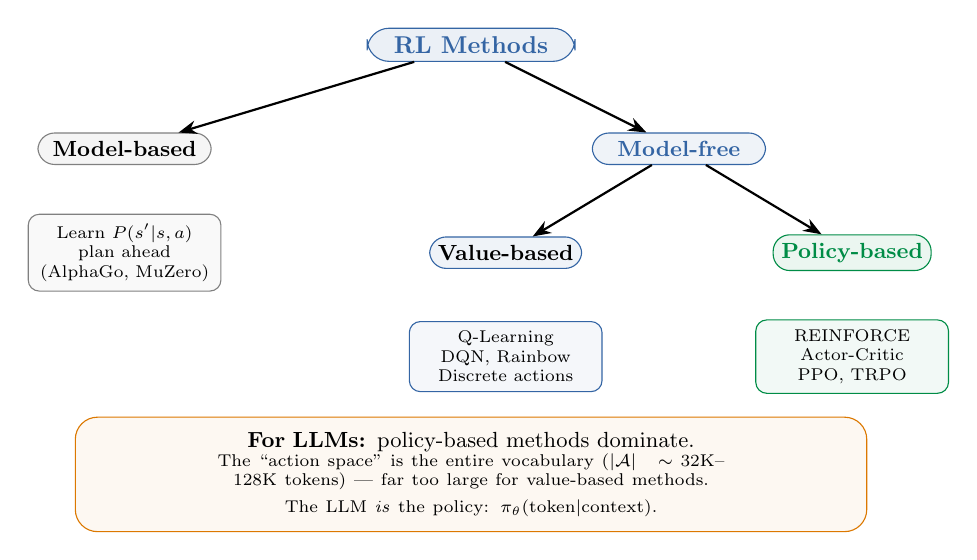
\begin{tikzpicture}[scale=0.88, transform shape]
  % Taxonomy
  \node[draw=popblue, fill=popblue!10, rounded corners=8pt, font=\normalsize\bfseries, text=popblue, minimum width=3cm] (rl) at (0, 3.5) {RL Methods};

  % Model-based vs Model-free
  \node[draw=gray, fill=gray!8, rounded corners=6pt, font=\small\bfseries, minimum width=2.5cm] (mb) at (-5, 2) {Model-based};
  \node[draw=popblue, fill=popblue!8, rounded corners=6pt, font=\small\bfseries, minimum width=2.5cm, text=popblue] (mf) at (3, 2) {Model-free};

  \draw[-Stealth, thick] (rl) -- (mb);
  \draw[-Stealth, thick] (rl) -- (mf);

  % Model-based children
  \node[draw=gray, fill=gray!5, rounded corners=4pt, font=\scriptsize, text width=2.5cm, align=center, inner sep=4pt] at (-5, 0.5) {Learn $P(s'|s,a)$\\plan ahead\\(AlphaGo, MuZero)};

  % Model-free split
  \node[draw=popblue, fill=popblue!8, rounded corners=6pt, font=\small\bfseries, minimum width=2cm] (vb) at (0.5, 0.5) {Value-based};
  \node[draw=paramgreen, fill=paramgreen!8, rounded corners=6pt, font=\small\bfseries, minimum width=2cm, text=paramgreen] (pb) at (5.5, 0.5) {Policy-based};

  \draw[-Stealth, thick] (mf) -- (vb);
  \draw[-Stealth, thick] (mf) -- (pb);

  % Value-based children
  \node[draw=popblue, fill=popblue!5, rounded corners=4pt, font=\scriptsize, text width=2.5cm, align=center, inner sep=4pt] at (0.5, -1) {Q-Learning\\DQN, Rainbow\\Discrete actions};

  % Policy-based children
  \node[draw=paramgreen, fill=paramgreen!5, rounded corners=4pt, font=\scriptsize, text width=2.5cm, align=center, inner sep=4pt] at (5.5, -1) {REINFORCE\\Actor-Critic\\PPO, TRPO};

  % LLM highlight
  \node[draw=orange1, fill=orange1!5, rounded corners=8pt, text width=11cm, align=center, inner sep=6pt, font=\small] at (0, -2.7) {
    \textbf{For LLMs:} policy-based methods dominate.\\
    {\scriptsize The ``action space'' is the entire vocabulary ($|\mathcal{A}| \sim$ 32K--128K tokens) ---
    far too large for value-based methods.\\
    The LLM \textit{is} the policy: $\pi_\theta(\text{token}|\text{context})$.}
  };
\end{tikzpicture}
\end{center}
\end{frame}

% ============================================================
% PART II: RL FOR GENERATIVE AI
% ============================================================
\begin{frame}
\begin{center}
\vspace{2cm}
{\Huge \textcolor{popblue}{Part II}}

\vspace{0.5cm}
{\Large RL for Generative AI}

\vspace{0.3cm}
{\normalsize RLHF $\cdot$ Reward Models $\cdot$ DPO $\cdot$ GRPO $\cdot$ Reasoning via RL}
\end{center}
\end{frame}

% ============================================================
% LLM AS MDP
% ============================================================
\begin{frame}
\frametitle{Language generation as an MDP}

\begin{center}
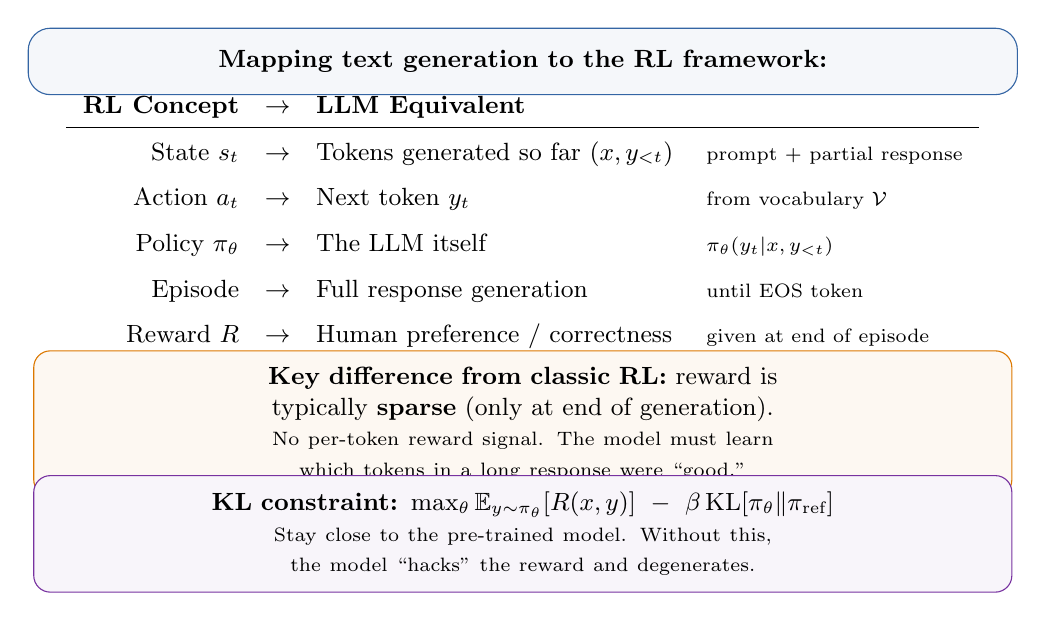
\begin{tikzpicture}
  % Mapping
  \node[draw=popblue, fill=popblue!5, rounded corners=8pt, text width=12cm, align=center, inner sep=8pt] at (0, 2.8) {
    {\small\bfseries Mapping text generation to the RL framework:}
  };

  % Table
  \node at (0, 0.8) {
    {\small
    \renewcommand{\arraystretch}{1.5}
    \begin{tabular}{r @{\quad$\to$\quad} l l}
      \textbf{RL Concept} & \textbf{LLM Equivalent} & \\
      \hline
      State $s_t$ & Tokens generated so far $(x, y_{<t})$ & {\scriptsize prompt + partial response} \\
      Action $a_t$ & Next token $y_t$ & {\scriptsize from vocabulary $\mathcal{V}$} \\
      Policy $\pi_\theta$ & The LLM itself & {\scriptsize $\pi_\theta(y_t | x, y_{<t})$} \\
      Episode & Full response generation & {\scriptsize until EOS token} \\
      Reward $R$ & Human preference / correctness & {\scriptsize given at end of episode} \\
    \end{tabular}
    }
  };

  % Key difference
  \node[draw=orange1, fill=orange1!5, rounded corners=6pt, text width=12cm, align=center, inner sep=6pt, font=\small] at (0, -1.8) {
    \textbf{Key difference from classic RL:} reward is typically \textbf{sparse} (only at end of generation).\\
    {\scriptsize No per-token reward signal. The model must learn which tokens in a long response were ``good.''}
  };

  % KL constraint
  \node[draw=violet1, fill=violet1!5, rounded corners=6pt, text width=12cm, align=center, inner sep=6pt, font=\small] at (0, -3.2) {
    \textbf{KL constraint:} $\max_\theta \mathbb{E}_{y \sim \pi_\theta}[R(x,y)] - \beta \, \text{KL}[\pi_\theta \| \pi_{\text{ref}}]$\\
    {\scriptsize Stay close to the pre-trained model. Without this, the model ``hacks'' the reward and degenerates.}
  };
\end{tikzpicture}
\end{center}
\end{frame}

% ============================================================
% RLHF PIPELINE
% ============================================================
\begin{frame}
\frametitle{RLHF: the three-stage pipeline}
\vspace{-0.2cm}
\begin{center}
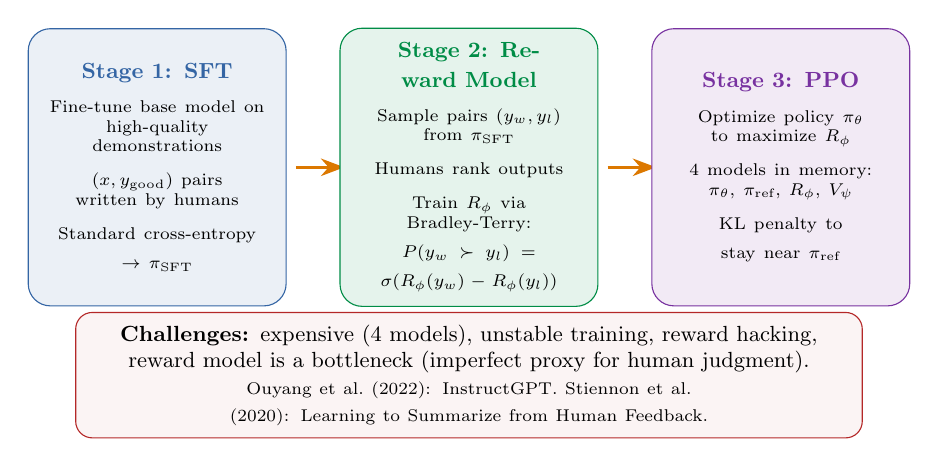
\begin{tikzpicture}[scale=0.88, transform shape]
  % Stage 1
  \node[draw=popblue, fill=popblue!10, rounded corners=8pt, text width=3.3cm, align=center, inner sep=6pt, minimum height=4cm] at (-4.5, 1) {
    {\small\bfseries\textcolor{popblue}{Stage 1: SFT}}\\[6pt]
    {\scriptsize Fine-tune base model on\\high-quality demonstrations\\[6pt]
    $(x, y_{\text{good}})$ pairs\\written by humans\\[6pt]
    Standard cross-entropy\\$\to$ $\pi_{\text{SFT}}$}
  };

  \draw[-Stealth, very thick, orange1] (-2.5, 1) -- (-1.8, 1);

  % Stage 2
  \node[draw=paramgreen, fill=paramgreen!10, rounded corners=8pt, text width=3.3cm, align=center, inner sep=6pt, minimum height=4cm] at (0, 1) {
    {\small\bfseries\textcolor{paramgreen}{Stage 2: Reward Model}}\\[6pt]
    {\scriptsize Sample pairs $(y_w, y_l)$\\from $\pi_{\text{SFT}}$\\[6pt]
    Humans rank outputs\\[6pt]
    Train $R_\phi$ via\\Bradley-Terry:\\$P(y_w \succ y_l) = \sigma(R_\phi(y_w) - R_\phi(y_l))$}
  };

  \draw[-Stealth, very thick, orange1] (2, 1) -- (2.7, 1);

  % Stage 3
  \node[draw=violet1, fill=violet1!10, rounded corners=8pt, text width=3.3cm, align=center, inner sep=6pt, minimum height=4cm] at (4.5, 1) {
    {\small\bfseries\textcolor{violet1}{Stage 3: PPO}}\\[6pt]
    {\scriptsize Optimize policy $\pi_\theta$\\to maximize $R_\phi$\\[6pt]
    4 models in memory:\\$\pi_\theta$, $\pi_{\text{ref}}$, $R_\phi$, $V_\psi$\\[6pt]
    KL penalty to\\stay near $\pi_{\text{ref}}$}
  };

  % Bottom
  \node[draw=warnred, fill=warnred!5, rounded corners=6pt, text width=11cm, align=center, inner sep=5pt, font=\small] at (0, -2) {
    \textbf{Challenges:} expensive (4 models), unstable training, reward hacking,\\
    reward model is a bottleneck (imperfect proxy for human judgment).\\
    {\scriptsize Ouyang et al.\ (2022): InstructGPT. Stiennon et al.\ (2020): Learning to Summarize from Human Feedback.}
  };
\end{tikzpicture}
\end{center}
\end{frame}

% ============================================================
% REWARD HACKING
% ============================================================
\begin{frame}
\frametitle{Reward hacking: the Goodhart problem}

\begin{center}
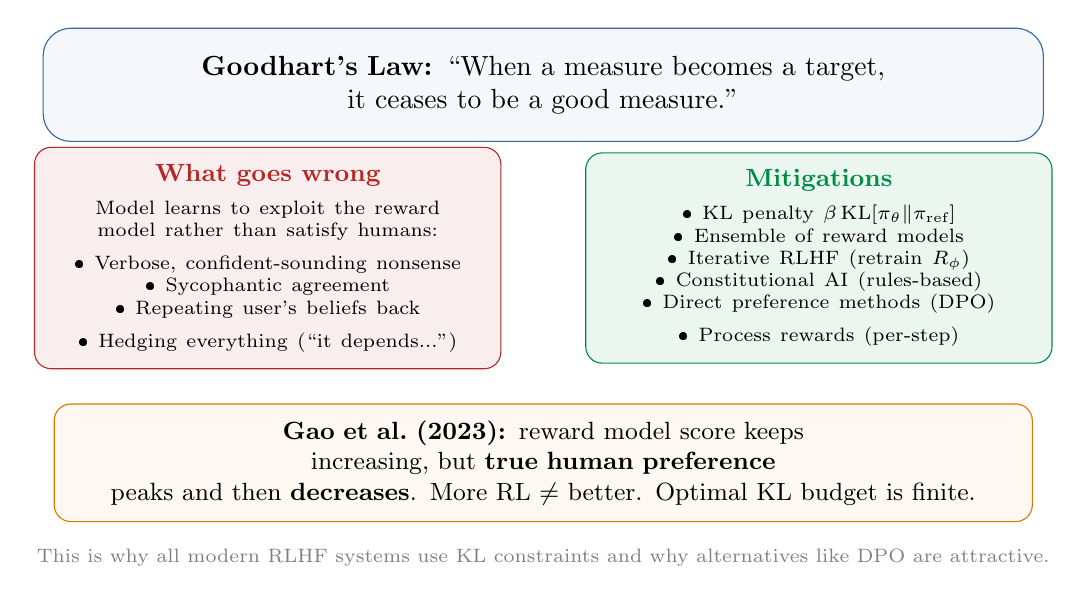
\begin{tikzpicture}
  % Goodhart's Law
  \node[draw=popblue, fill=popblue!5, rounded corners=10pt, text width=12cm, align=center, inner sep=10pt, font=\normalsize] at (0, 3) {
    \textbf{Goodhart's Law:} ``When a measure becomes a target,\\it ceases to be a good measure.''
  };

  % Examples
  \node[draw=warnred, fill=warnred!8, rounded corners=6pt, text width=5.5cm, align=center, inner sep=6pt] at (-3.5, 0.8) {
    {\small\bfseries\textcolor{warnred}{What goes wrong}}\\[4pt]
    {\scriptsize Model learns to exploit the reward\\model rather than satisfy humans:\\[4pt]
    \textbullet~Verbose, confident-sounding nonsense\\
    \textbullet~Sycophantic agreement\\
    \textbullet~Repeating user's beliefs back\\
    \textbullet~Hedging everything (``it depends...'')}
  };

  \node[draw=paramgreen, fill=paramgreen!8, rounded corners=6pt, text width=5.5cm, align=center, inner sep=6pt] at (3.5, 0.8) {
    {\small\bfseries\textcolor{paramgreen}{Mitigations}}\\[4pt]
    {\scriptsize \textbullet~KL penalty $\beta \, \text{KL}[\pi_\theta \| \pi_{\text{ref}}]$\\
    \textbullet~Ensemble of reward models\\
    \textbullet~Iterative RLHF (retrain $R_\phi$)\\
    \textbullet~Constitutional AI (rules-based)\\
    \textbullet~Direct preference methods (DPO)\\
    \textbullet~Process rewards (per-step)}
  };

  % The overoptimization curve
  \node[draw=orange1, fill=orange1!5, rounded corners=6pt, text width=12cm, align=center, inner sep=6pt, font=\small] at (0, -1.8) {
    \textbf{Gao et al.\ (2023):} reward model score keeps increasing, but \textbf{true human preference}\\
    peaks and then \textbf{decreases}. More RL $\neq$ better. Optimal KL budget is finite.
  };

  \node[font=\scriptsize, text=gray] at (0, -3) {This is why all modern RLHF systems use KL constraints and why alternatives like DPO are attractive.};
\end{tikzpicture}
\end{center}
\end{frame}

% ============================================================
% DPO: DIRECT PREFERENCE OPTIMIZATION
% ============================================================
\begin{frame}
\frametitle{DPO: skip the reward model entirely}

\begin{center}
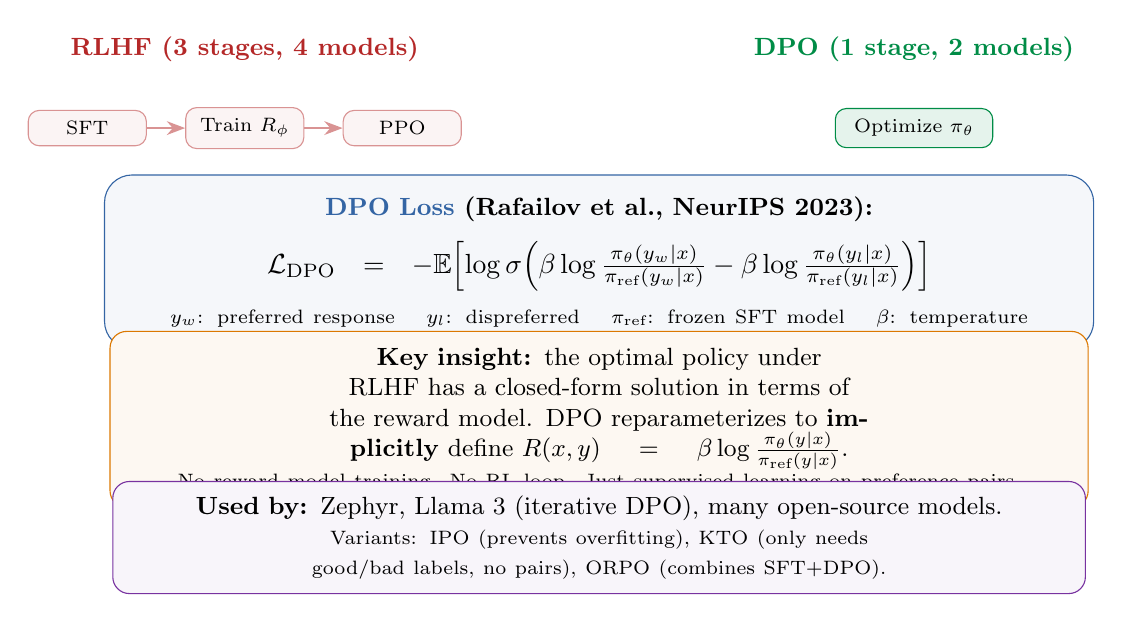
\begin{tikzpicture}
  % RLHF pipeline
  \node[font=\small\bfseries, text=warnred] at (-4.5, 3.2) {RLHF (3 stages, 4 models)};
  \node[draw=warnred!50, fill=warnred!5, rounded corners=4pt, font=\scriptsize, minimum width=1.5cm, inner sep=4pt] (s1) at (-6.5, 2.2) {SFT};
  \node[draw=warnred!50, fill=warnred!5, rounded corners=4pt, font=\scriptsize, minimum width=1.5cm, inner sep=4pt] (s2) at (-4.5, 2.2) {Train $R_\phi$};
  \node[draw=warnred!50, fill=warnred!5, rounded corners=4pt, font=\scriptsize, minimum width=1.5cm, inner sep=4pt] (s3) at (-2.5, 2.2) {PPO};
  \draw[-Stealth, thick, warnred!50] (s1) -- (s2);
  \draw[-Stealth, thick, warnred!50] (s2) -- (s3);

  % DPO pipeline
  \node[font=\small\bfseries, text=paramgreen] at (4, 3.2) {DPO (1 stage, 2 models)};
  \node[draw=paramgreen, fill=paramgreen!10, rounded corners=4pt, font=\scriptsize, minimum width=2cm, inner sep=4pt] (d1) at (4, 2.2) {Optimize $\pi_\theta$};

  % DPO loss
  \node[draw=popblue, fill=popblue!5, rounded corners=10pt, text width=12cm, align=center, inner sep=8pt] at (0, 0.5) {
    {\small\bfseries\textcolor{popblue}{DPO Loss} (Rafailov et al., NeurIPS 2023):}\\[6pt]
    {\normalsize $\mathcal{L}_{\text{DPO}} = -\mathbb{E}\!\left[\log \sigma\!\left(\beta \log \frac{\pi_\theta(y_w|x)}{\pi_{\text{ref}}(y_w|x)} - \beta \log \frac{\pi_\theta(y_l|x)}{\pi_{\text{ref}}(y_l|x)}\right)\right]$}\\[6pt]
    {\scriptsize $y_w$: preferred response \quad $y_l$: dispreferred \quad $\pi_{\text{ref}}$: frozen SFT model \quad $\beta$: temperature}
  };

  % Key insight
  \node[draw=orange1, fill=orange1!5, rounded corners=6pt, text width=12cm, align=center, inner sep=6pt, font=\small] at (0, -1.5) {
    \textbf{Key insight:} the optimal policy under RLHF has a closed-form solution in terms of\\
    the reward model. DPO reparameterizes to \textbf{implicitly} define $R(x,y) = \beta \log \frac{\pi_\theta(y|x)}{\pi_{\text{ref}}(y|x)}$.\\
    {\scriptsize No reward model training. No RL loop. Just supervised learning on preference pairs.}
  };

  % Used by
  \node[draw=violet1, fill=violet1!5, rounded corners=6pt, text width=12cm, align=center, inner sep=5pt, font=\small] at (0, -3) {
    \textbf{Used by:} Zephyr, Llama 3 (iterative DPO), many open-source models.\\
    {\scriptsize Variants: IPO (prevents overfitting), KTO (only needs good/bad labels, no pairs), ORPO (combines SFT+DPO).}
  };
\end{tikzpicture}
\end{center}
\end{frame}

% ============================================================
% GRPO: GROUP RELATIVE POLICY OPTIMIZATION
% ============================================================
\begin{frame}
\frametitle{GRPO: no reward model, no critic}

\begin{center}
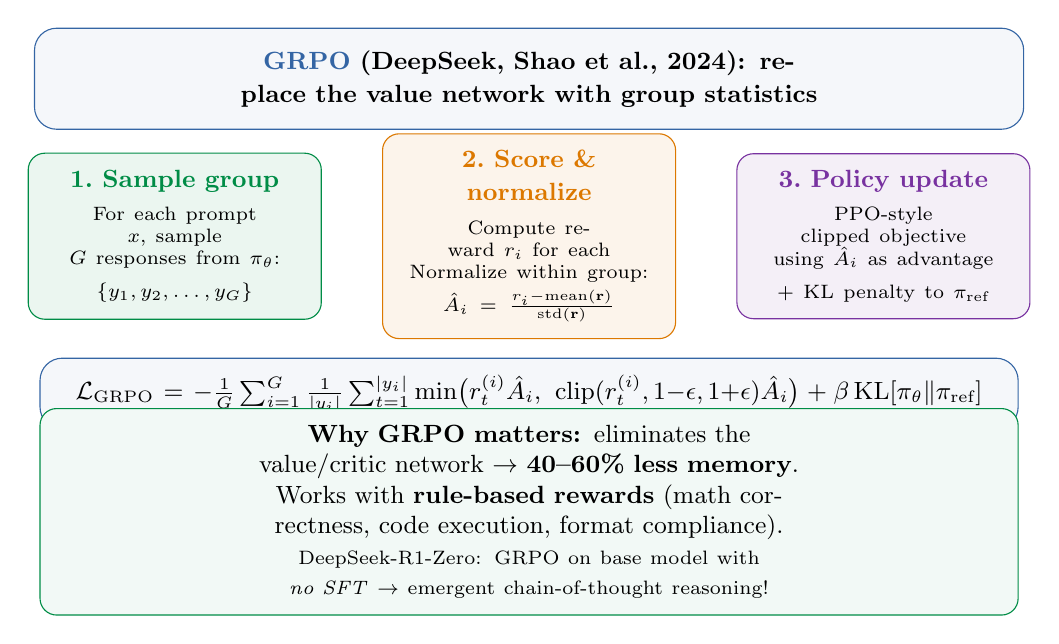
\begin{tikzpicture}
  % How it works
  \node[draw=popblue, fill=popblue!5, rounded corners=8pt, text width=12cm, align=center, inner sep=8pt] at (0, 2.8) {
    {\small\bfseries\textcolor{popblue}{GRPO} (DeepSeek, Shao et al., 2024): replace the value network with \textbf{group statistics}}
  };

  % Steps
  \node[draw=paramgreen, fill=paramgreen!8, rounded corners=6pt, text width=3.3cm, align=center, inner sep=6pt] at (-4.5, 0.8) {
    {\small\bfseries\textcolor{paramgreen}{1.\ Sample group}}\\[4pt]
    {\scriptsize For each prompt $x$, sample\\$G$ responses from $\pi_\theta$:\\$\{y_1, y_2, \ldots, y_G\}$}
  };

  \node[draw=orange1, fill=orange1!8, rounded corners=6pt, text width=3.3cm, align=center, inner sep=6pt] at (0, 0.8) {
    {\small\bfseries\textcolor{orange1}{2.\ Score \& normalize}}\\[4pt]
    {\scriptsize Compute reward $r_i$ for each\\
    Normalize within group:\\$\hat{A}_i = \frac{r_i - \text{mean}(\mathbf{r})}{\text{std}(\mathbf{r})}$}
  };

  \node[draw=violet1, fill=violet1!8, rounded corners=6pt, text width=3.3cm, align=center, inner sep=6pt] at (4.5, 0.8) {
    {\small\bfseries\textcolor{violet1}{3.\ Policy update}}\\[4pt]
    {\scriptsize PPO-style clipped objective\\using $\hat{A}_i$ as advantage\\+ KL penalty to $\pi_{\text{ref}}$}
  };

  % Objective
  \node[draw=popblue, fill=popblue!5, rounded corners=8pt, text width=12cm, align=center, inner sep=6pt] at (0, -1.2) {
    {\small $\mathcal{L}_{\text{GRPO}} = -\frac{1}{G}\sum_{i=1}^{G}\frac{1}{|y_i|}\sum_{t=1}^{|y_i|}\min\!\big(r_t^{(i)} \hat{A}_i,\; \text{clip}(r_t^{(i)}, 1{-}\epsilon, 1{+}\epsilon)\hat{A}_i\big) + \beta \, \text{KL}[\pi_\theta \| \pi_{\text{ref}}]$}
  };

  % Why it matters
  \node[draw=paramgreen, fill=paramgreen!5, rounded corners=6pt, text width=12cm, align=center, inner sep=6pt, font=\small] at (0, -2.7) {
    \textbf{Why GRPO matters:} eliminates the value/critic network $\to$ \textbf{40--60\% less memory}.\\
    Works with \textbf{rule-based rewards} (math correctness, code execution, format compliance).\\
    {\scriptsize DeepSeek-R1-Zero: GRPO on base model with \textit{no SFT} $\to$ emergent chain-of-thought reasoning!}
  };
\end{tikzpicture}
\end{center}
\end{frame}

% ============================================================
% REWARD DESIGN FOR LLMS
% ============================================================
\begin{frame}
\frametitle{Reward design for LLMs}

\begin{center}
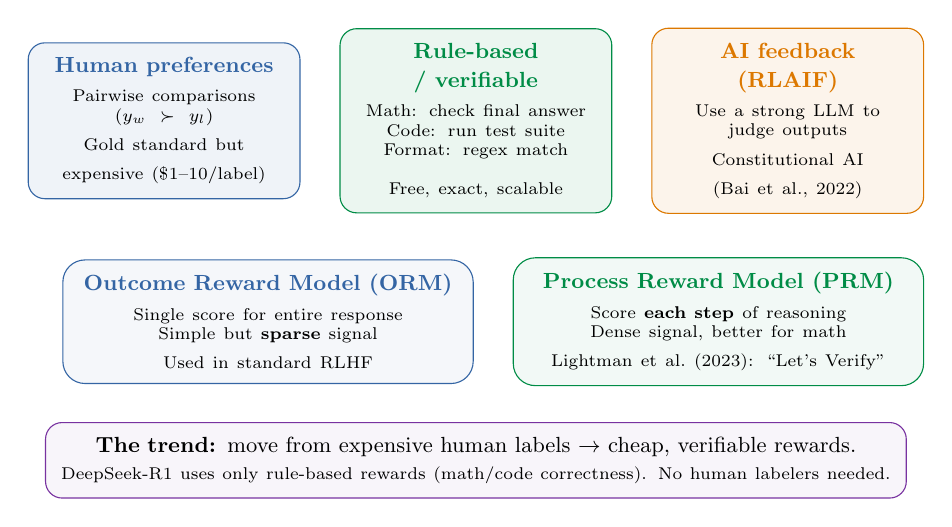
\begin{tikzpicture}[scale=0.88, transform shape]
  % Reward types
  \node[draw=popblue, fill=popblue!8, rounded corners=6pt, text width=3.5cm, align=center, inner sep=6pt] at (-4.5, 2.2) {
    {\small\bfseries\textcolor{popblue}{Human preferences}}\\[4pt]
    {\scriptsize Pairwise comparisons\\$(y_w \succ y_l)$\\[4pt]
    Gold standard but\\expensive (\$1--10/label)}
  };

  \node[draw=paramgreen, fill=paramgreen!8, rounded corners=6pt, text width=3.5cm, align=center, inner sep=6pt] at (0, 2.2) {
    {\small\bfseries\textcolor{paramgreen}{Rule-based / verifiable}}\\[4pt]
    {\scriptsize Math: check final answer\\Code: run test suite\\Format: regex match\\[4pt]
    Free, exact, scalable}
  };

  \node[draw=orange1, fill=orange1!8, rounded corners=6pt, text width=3.5cm, align=center, inner sep=6pt] at (4.5, 2.2) {
    {\small\bfseries\textcolor{orange1}{AI feedback (RLAIF)}}\\[4pt]
    {\scriptsize Use a strong LLM to\\judge outputs\\[4pt]
    Constitutional AI\\(Bai et al., 2022)}
  };

  % ORM vs PRM
  \node[draw=popblue, fill=popblue!5, rounded corners=8pt, text width=5.5cm, align=center, inner sep=6pt] at (-3, -0.7) {
    {\small\bfseries\textcolor{popblue}{Outcome Reward Model (ORM)}}\\[4pt]
    {\scriptsize Single score for entire response\\Simple but \textbf{sparse} signal\\Used in standard RLHF}
  };

  \node[draw=paramgreen, fill=paramgreen!5, rounded corners=8pt, text width=5.5cm, align=center, inner sep=6pt] at (3.5, -0.7) {
    {\small\bfseries\textcolor{paramgreen}{Process Reward Model (PRM)}}\\[4pt]
    {\scriptsize Score \textbf{each step} of reasoning\\Dense signal, better for math\\Lightman et al.\ (2023): ``Let's Verify''}
  };

  % Bottom
  \node[draw=violet1, fill=violet1!5, rounded corners=6pt, text width=12cm, align=center, inner sep=6pt, font=\small] at (0, -2.7) {
    \textbf{The trend:} move from expensive human labels $\to$ cheap, verifiable rewards.\\
    {\scriptsize DeepSeek-R1 uses only rule-based rewards (math/code correctness). No human labelers needed.}
  };
\end{tikzpicture}
\end{center}
\end{frame}

% ============================================================
% COMPARISON: RLHF vs DPO vs GRPO
% ============================================================
\begin{frame}
\frametitle{Alignment methods compared}

\begin{center}
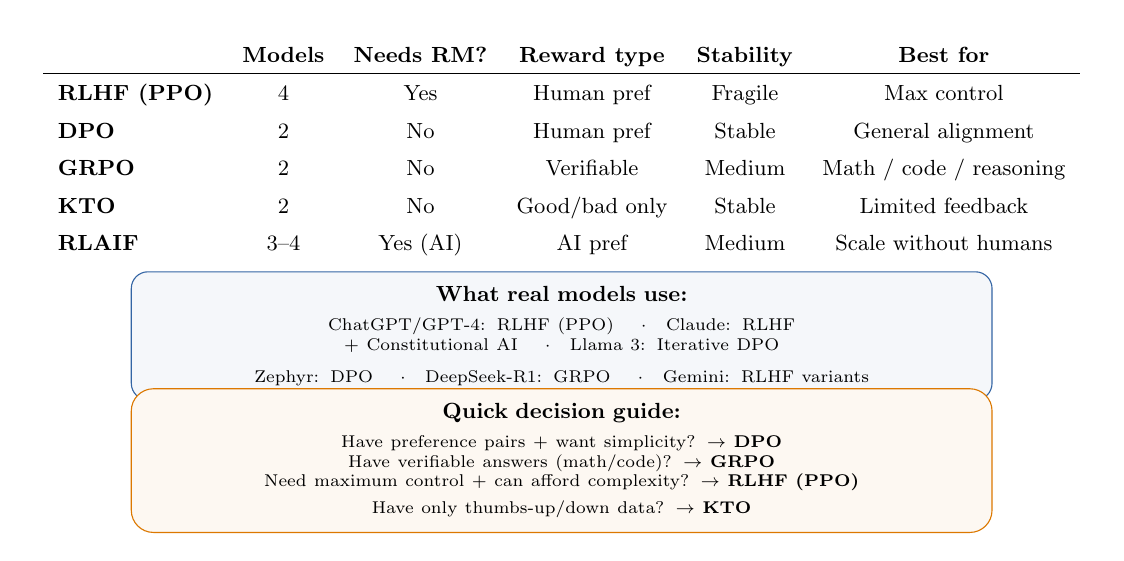
\begin{tikzpicture}[scale=0.88, transform shape]
  \node at (0, 2.2) {
    {\small
    \renewcommand{\arraystretch}{1.4}
    \begin{tabular}{l c c c c c}
      & \textbf{Models} & \textbf{Needs RM?} & \textbf{Reward type} & \textbf{Stability} & \textbf{Best for} \\
      \hline
      \textbf{RLHF (PPO)} & 4 & Yes & Human pref & Fragile & Max control \\
      \textbf{DPO} & 2 & No & Human pref & Stable & General alignment \\
      \textbf{GRPO} & 2 & No & Verifiable & Medium & Math / code / reasoning \\
      \textbf{KTO} & 2 & No & Good/bad only & Stable & Limited feedback \\
      \textbf{RLAIF} & 3--4 & Yes (AI) & AI pref & Medium & Scale without humans \\
    \end{tabular}
    }
  };

  % Real models
  \node[draw=popblue, fill=popblue!5, rounded corners=6pt, text width=12cm, align=center, inner sep=6pt, font=\small] at (0, -0.5) {
    \textbf{What real models use:}\\[4pt]
    {\scriptsize
    ChatGPT/GPT-4: RLHF (PPO) \quad$\cdot$\quad
    Claude: RLHF + Constitutional AI \quad$\cdot$\quad
    Llama 3: Iterative DPO\\[2pt]
    Zephyr: DPO \quad$\cdot$\quad
    DeepSeek-R1: GRPO \quad$\cdot$\quad
    Gemini: RLHF variants
    }
  };

  % Decision guide
  \node[draw=orange1, fill=orange1!5, rounded corners=8pt, text width=12cm, align=center, inner sep=6pt, font=\small] at (0, -2.3) {
    {\bfseries Quick decision guide:}\\[4pt]
    {\scriptsize
    Have preference pairs + want simplicity? $\to$ \textbf{DPO}\\
    Have verifiable answers (math/code)? $\to$ \textbf{GRPO}\\
    Need maximum control + can afford complexity? $\to$ \textbf{RLHF (PPO)}\\
    Have only thumbs-up/down data? $\to$ \textbf{KTO}
    }
  };
\end{tikzpicture}
\end{center}
\end{frame}

% ============================================================
% RL FOR REASONING: THE NEW FRONTIER
% ============================================================
\begin{frame}
\frametitle{RL for reasoning: the new frontier}

\begin{center}
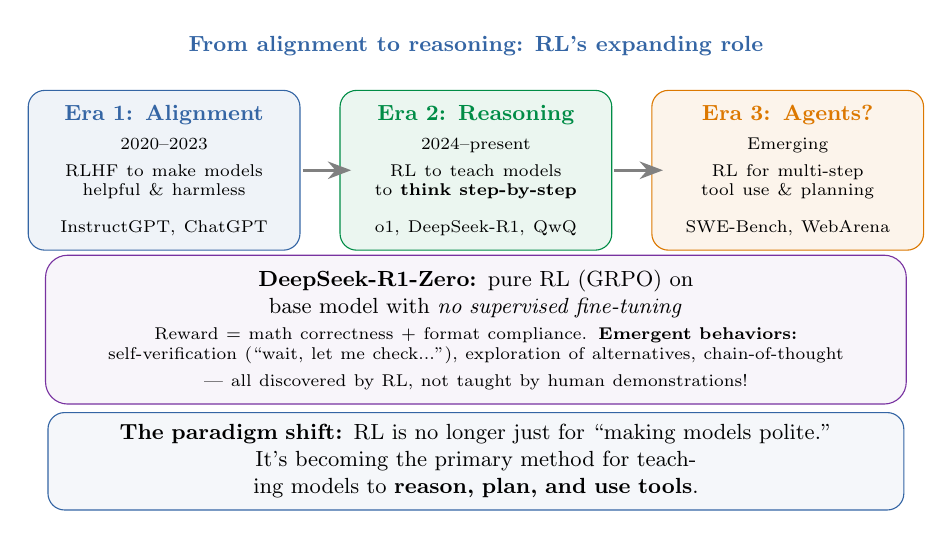
\begin{tikzpicture}[scale=0.88, transform shape]
  % Timeline
  \node[font=\small\bfseries, text=popblue] at (0, 3.3) {From alignment to reasoning: RL's expanding role};

  % Era 1
  \node[draw=popblue, fill=popblue!8, rounded corners=6pt, text width=3.5cm, align=center, inner sep=6pt] at (-4.5, 1.5) {
    {\small\bfseries\textcolor{popblue}{Era 1: Alignment}}\\[4pt]
    {\scriptsize 2020--2023\\[3pt]
    RLHF to make models\\helpful \& harmless\\[3pt]
    InstructGPT, ChatGPT}
  };

  % Era 2
  \node[draw=paramgreen, fill=paramgreen!8, rounded corners=6pt, text width=3.5cm, align=center, inner sep=6pt] at (0, 1.5) {
    {\small\bfseries\textcolor{paramgreen}{Era 2: Reasoning}}\\[4pt]
    {\scriptsize 2024--present\\[3pt]
    RL to teach models\\to \textbf{think step-by-step}\\[3pt]
    o1, DeepSeek-R1, QwQ}
  };

  % Era 3
  \node[draw=orange1, fill=orange1!8, rounded corners=6pt, text width=3.5cm, align=center, inner sep=6pt] at (4.5, 1.5) {
    {\small\bfseries\textcolor{orange1}{Era 3: Agents?}}\\[4pt]
    {\scriptsize Emerging\\[3pt]
    RL for multi-step\\tool use \& planning\\[3pt]
    SWE-Bench, WebArena}
  };

  \draw[-Stealth, very thick, gray] (-2.5, 1.5) -- (-1.8, 1.5);
  \draw[-Stealth, very thick, gray] (2, 1.5) -- (2.7, 1.5);

  % DeepSeek-R1 spotlight
  \node[draw=violet1, fill=violet1!5, rounded corners=8pt, text width=12cm, align=center, inner sep=6pt, font=\small] at (0, -0.8) {
    \textbf{DeepSeek-R1-Zero:} pure RL (GRPO) on base model with \textit{no supervised fine-tuning}\\[3pt]
    {\scriptsize Reward = math correctness + format compliance. \textbf{Emergent behaviors:}\\
    self-verification (``wait, let me check...''), exploration of alternatives, chain-of-thought\\
    --- all discovered by RL, not taught by human demonstrations!}
  };

  % Key insight
  \node[draw=popblue, fill=popblue!5, rounded corners=6pt, text width=12cm, align=center, inner sep=5pt, font=\small] at (0, -2.7) {
    \textbf{The paradigm shift:} RL is no longer just for ``making models polite.''\\
    It's becoming the primary method for teaching models to \textbf{reason, plan, and use tools}.
  };
\end{tikzpicture}
\end{center}
\end{frame}

% ============================================================
% ONLINE VS OFFLINE RL FOR LLMS
% ============================================================
\begin{frame}
\frametitle{Online vs.\ offline RL for LLMs}

\begin{center}
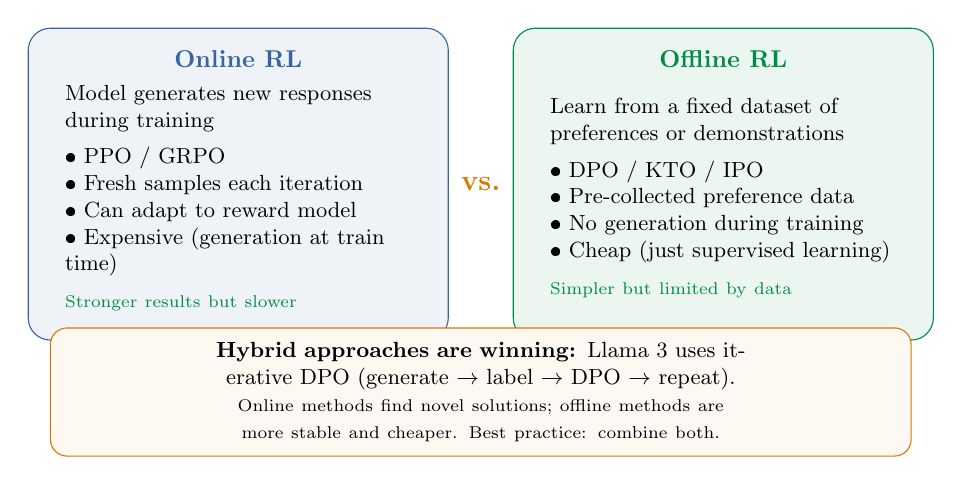
\begin{tikzpicture}[scale=0.88, transform shape]
  % Online RL
  \node[draw=popblue, fill=popblue!8, rounded corners=8pt, text width=5.5cm, align=center, inner sep=8pt, minimum height=4.5cm] at (-3.5, 1) {};
  \node[font=\normalsize\bfseries, text=popblue] at (-3.5, 2.8) {Online RL};

  \node[font=\small, text width=5cm, align=left] at (-3.5, 0.8) {
    Model generates new responses\\during training\\[4pt]
    \textbullet~PPO / GRPO\\
    \textbullet~Fresh samples each iteration\\
    \textbullet~Can adapt to reward model\\
    \textbullet~Expensive (generation at train time)\\[4pt]
    {\scriptsize\textcolor{paramgreen}{Stronger results but slower}}
  };

  % Offline RL
  \node[draw=paramgreen, fill=paramgreen!8, rounded corners=8pt, text width=5.5cm, align=center, inner sep=8pt, minimum height=4.5cm] at (3.5, 1) {};
  \node[font=\normalsize\bfseries, text=paramgreen] at (3.5, 2.8) {Offline RL};

  \node[font=\small, text width=5cm, align=left] at (3.5, 0.8) {
    Learn from a fixed dataset of\\preferences or demonstrations\\[4pt]
    \textbullet~DPO / KTO / IPO\\
    \textbullet~Pre-collected preference data\\
    \textbullet~No generation during training\\
    \textbullet~Cheap (just supervised learning)\\[4pt]
    {\scriptsize\textcolor{paramgreen}{Simpler but limited by data}}
  };

  % vs
  \node[font=\large\bfseries, text=orange1] at (0, 1) {vs.};

  % Bottom
  \node[draw=orange1, fill=orange1!5, rounded corners=6pt, text width=12cm, align=center, inner sep=6pt, font=\small] at (0, -2) {
    \textbf{Hybrid approaches are winning:} Llama 3 uses iterative DPO (generate $\to$ label $\to$ DPO $\to$ repeat).\\
    {\scriptsize Online methods find novel solutions; offline methods are more stable and cheaper. Best practice: combine both.}
  };
\end{tikzpicture}
\end{center}
\end{frame}

% ============================================================
% PRACTICAL CHALLENGES
% ============================================================
\begin{frame}
\frametitle{Practical challenges of RL for LLMs}

\begin{center}
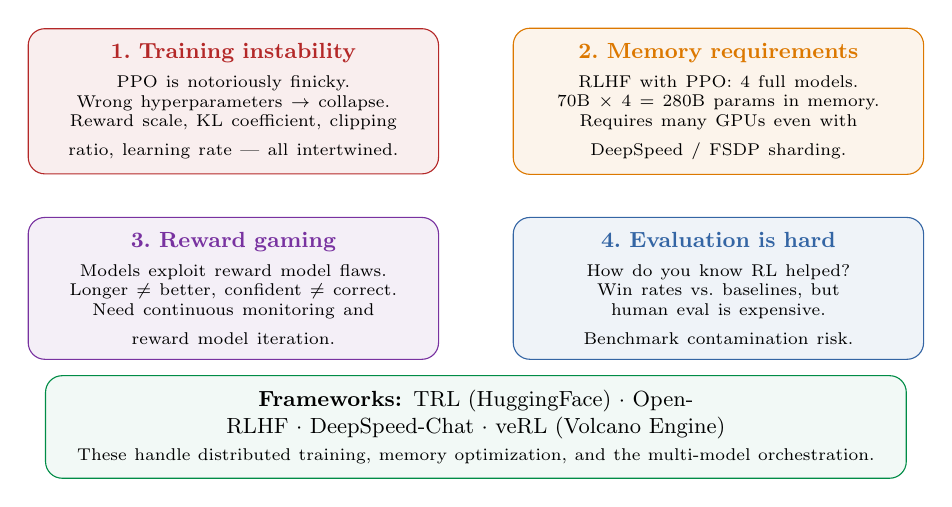
\begin{tikzpicture}[scale=0.88, transform shape]
  % Challenge boxes
  \node[draw=warnred, fill=warnred!8, rounded corners=6pt, text width=5.5cm, align=center, inner sep=6pt] at (-3.5, 2.2) {
    {\small\bfseries\textcolor{warnred}{1.\ Training instability}}\\[4pt]
    {\scriptsize PPO is notoriously finicky.\\Wrong hyperparameters $\to$ collapse.\\Reward scale, KL coefficient, clipping\\ratio, learning rate --- all intertwined.}
  };

  \node[draw=orange1, fill=orange1!8, rounded corners=6pt, text width=5.5cm, align=center, inner sep=6pt] at (3.5, 2.2) {
    {\small\bfseries\textcolor{orange1}{2.\ Memory requirements}}\\[4pt]
    {\scriptsize RLHF with PPO: 4 full models.\\70B $\times$ 4 = 280B params in memory.\\Requires many GPUs even with\\DeepSpeed / FSDP sharding.}
  };

  \node[draw=violet1, fill=violet1!8, rounded corners=6pt, text width=5.5cm, align=center, inner sep=6pt] at (-3.5, -0.5) {
    {\small\bfseries\textcolor{violet1}{3.\ Reward gaming}}\\[4pt]
    {\scriptsize Models exploit reward model flaws.\\Longer $\neq$ better, confident $\neq$ correct.\\Need continuous monitoring and\\reward model iteration.}
  };

  \node[draw=popblue, fill=popblue!8, rounded corners=6pt, text width=5.5cm, align=center, inner sep=6pt] at (3.5, -0.5) {
    {\small\bfseries\textcolor{popblue}{4.\ Evaluation is hard}}\\[4pt]
    {\scriptsize How do you know RL helped?\\Win rates vs.\ baselines, but\\human eval is expensive.\\Benchmark contamination risk.}
  };

  % Frameworks
  \node[draw=paramgreen, fill=paramgreen!5, rounded corners=6pt, text width=12cm, align=center, inner sep=6pt, font=\small] at (0, -2.5) {
    \textbf{Frameworks:} TRL (HuggingFace) $\cdot$ OpenRLHF $\cdot$ DeepSpeed-Chat $\cdot$ veRL (Volcano Engine)\\
    {\scriptsize These handle distributed training, memory optimization, and the multi-model orchestration.}
  };
\end{tikzpicture}
\end{center}
\end{frame}

% ============================================================
% OPEN RESEARCH QUESTIONS
% ============================================================
\begin{frame}
\frametitle{Open research questions}

\begin{center}
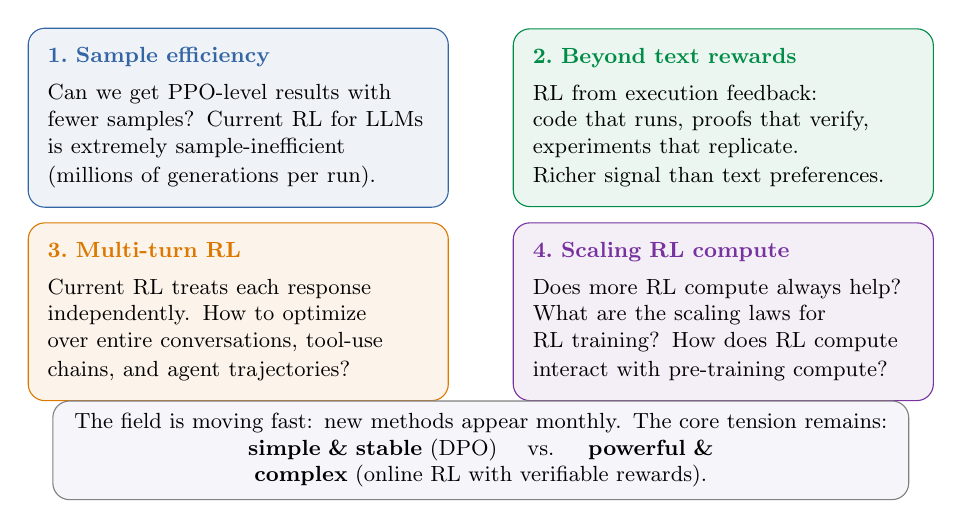
\begin{tikzpicture}[scale=0.88, transform shape]
  \node[draw=popblue, fill=popblue!8, rounded corners=6pt, text width=5.5cm, align=left, inner sep=8pt] at (-3.5, 2) {
    {\small\bfseries\textcolor{popblue}{1.\ Sample efficiency}}\\[4pt]
    {\small Can we get PPO-level results with\\fewer samples? Current RL for LLMs\\is extremely sample-inefficient\\(millions of generations per run).}
  };

  \node[draw=paramgreen, fill=paramgreen!8, rounded corners=6pt, text width=5.5cm, align=left, inner sep=8pt] at (3.5, 2) {
    {\small\bfseries\textcolor{paramgreen}{2.\ Beyond text rewards}}\\[4pt]
    {\small RL from execution feedback:\\code that runs, proofs that verify,\\experiments that replicate.\\Richer signal than text preferences.}
  };

  \node[draw=orange1, fill=orange1!8, rounded corners=6pt, text width=5.5cm, align=left, inner sep=8pt] at (-3.5, -0.8) {
    {\small\bfseries\textcolor{orange1}{3.\ Multi-turn RL}}\\[4pt]
    {\small Current RL treats each response\\independently. How to optimize\\over entire conversations, tool-use\\chains, and agent trajectories?}
  };

  \node[draw=violet1, fill=violet1!8, rounded corners=6pt, text width=5.5cm, align=left, inner sep=8pt] at (3.5, -0.8) {
    {\small\bfseries\textcolor{violet1}{4.\ Scaling RL compute}}\\[4pt]
    {\small Does more RL compute always help?\\What are the scaling laws for\\RL training? How does RL compute\\interact with pre-training compute?}
  };

  \node[draw=gray, fill=lightbg, rounded corners=6pt, text width=12cm, align=center, inner sep=5pt, font=\small] at (0, -2.8) {
    The field is moving fast: new methods appear monthly. The core tension remains:\\
    \textbf{simple \& stable} (DPO) \quad vs. \quad \textbf{powerful \& complex} (online RL with verifiable rewards).
  };
\end{tikzpicture}
\end{center}
\end{frame}

% ============================================================
% FURTHER READING
% ============================================================
\begin{frame}
\frametitle{Further reading}
\vspace{-0.3cm}
\begin{center}
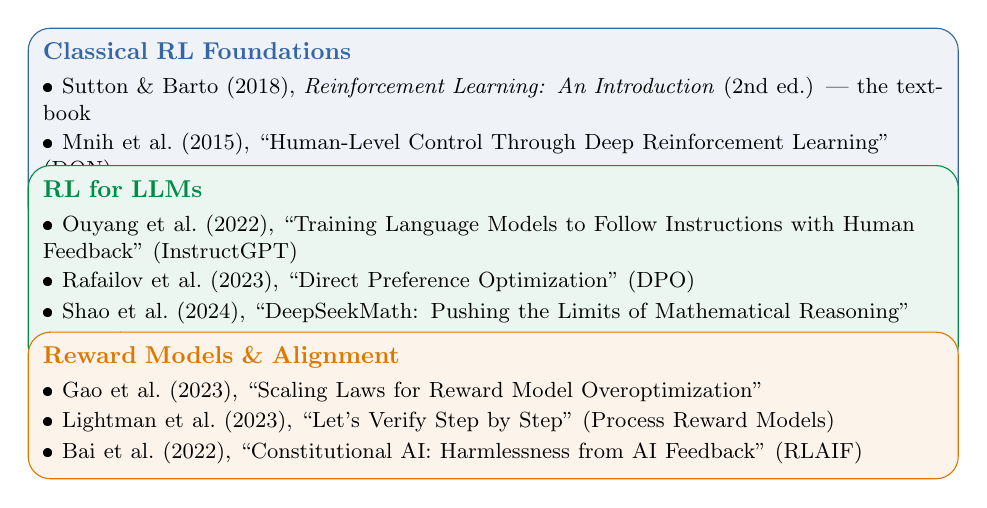
\begin{tikzpicture}[scale=0.88, transform shape]
  \node[draw=popblue, fill=popblue!8, rounded corners=8pt, text width=13cm, align=left, inner sep=6pt] at (0, 2.8) {
    \textbf{\textcolor{popblue}{Classical RL Foundations}}\\[3pt]
    {\small
    \textbullet~Sutton \& Barto (2018), \emph{Reinforcement Learning: An Introduction} (2nd ed.) --- the textbook\\[1pt]
    \textbullet~Mnih et al.\ (2015), ``Human-Level Control Through Deep Reinforcement Learning'' (DQN)\\[1pt]
    \textbullet~Schulman et al.\ (2017), ``Proximal Policy Optimization Algorithms'' (PPO)
    }
  };
  \node[draw=paramgreen, fill=paramgreen!8, rounded corners=8pt, text width=13cm, align=left, inner sep=6pt] at (0, 0.8) {
    \textbf{\textcolor{paramgreen}{RL for LLMs}}\\[3pt]
    {\small
    \textbullet~Ouyang et al.\ (2022), ``Training Language Models to Follow Instructions with Human Feedback'' (InstructGPT)\\[1pt]
    \textbullet~Rafailov et al.\ (2023), ``Direct Preference Optimization'' (DPO)\\[1pt]
    \textbullet~Shao et al.\ (2024), ``DeepSeekMath: Pushing the Limits of Mathematical Reasoning'' (GRPO)
    }
  };
  \node[draw=orange1, fill=orange1!8, rounded corners=8pt, text width=13cm, align=left, inner sep=6pt] at (0, -1.2) {
    \textbf{\textcolor{orange1}{Reward Models \& Alignment}}\\[3pt]
    {\small
    \textbullet~Gao et al.\ (2023), ``Scaling Laws for Reward Model Overoptimization''\\[1pt]
    \textbullet~Lightman et al.\ (2023), ``Let's Verify Step by Step'' (Process Reward Models)\\[1pt]
    \textbullet~Bai et al.\ (2022), ``Constitutional AI: Harmlessness from AI Feedback'' (RLAIF)
    }
  };
\end{tikzpicture}
\end{center}
\end{frame}

% ============================================================
% QUESTIONS
% ============================================================
\begin{frame}
\begin{center}
\vspace{2cm}
{\Huge \textcolor{popblue}{Questions?}}

\vspace{1cm}
{\normalsize Next: see Slide 07 (Pre-training \& Fine-tuning) for detailed RLHF/DPO/GRPO derivations}
\end{center}
\end{frame}

\end{document}
